\chapter{Tune procedure, CP5 Tune and \textsc{mcnntunes}}
\label{chap:TuneprocedureCP5TuneandMCNNTUNES}

The study of the underlying event, or more in general of softQCD processes require the use of Monte Carlo generator that often are based on phenomenological model with a lot of free parameters. These free parameters must be tuned on experimental data in order to obtain meaningful results from the simulations. The procedure of estimate the best parameters values is called \textit{tune}. 
\\
The tune procedure can be really computational expensive, in fact it requires to run the generator a very large amount of times, and usually these MC generators are really expansive in term of computational time required for just a single job.  
\\
To tune a certain number of parameters the number of jobs you have to run increase with this number of parameters, in fact the parameter space dimension increase with the number and the granularity of the sampling we want to perform. Different approaches have been developed and used in the past to tune these MC generators. A brief description is reported for each approach in the following list:
\begin{enumerate}[label=\arabic*)]
	\item \textbf{Manual tunes}: this approach is based on an optimization of the parameters made by eye. This is absolutely not the best way to tune some parameters, usually it requires a very large time for even semi-reasonable results since the process require a very large number of iterations .   
	\item \textbf{Brute force tunes}: a better way would be to perform a very dense sampling in parameters space and run the generator with every configuration. This is very computational expensive and a scan in a $5$ parameters space with $10$ division each requires $10^5=100000$ Monte Carlo runs this with a rising number of parameters becomes really impractical, also using computers batch systems as an example CondorHT (\textsc{cern}).   
	\item \textbf{Parametrization-based tunes}: an even more better approach is to find a surrogate function to parameterize the response of the MC generator at different values of the parameters to tune and try to study (minimize) this surrogate function instead of the real response of the generator. This is the right approach that is used in the high energy physics tune and that we are going to use in the follow for our tune.
\end{enumerate}
Let us discuss this last approach with more details in the next section.

\section{Parametrization-based approach}

The parametrization-based approach is the most used method. The current state-of-art in the tune procedure is to use a polynomial function to fit the response of the generator. Once the parametrization is performed the tuned parameters are given by the minimization of this parameterized response function. This approach based on the polynomial parametrization have been  implemented in the software \textsc{Professor} \cite{Buckley:2009bj}. 
\\
So the first step in the procedure is to fit the response of the generator using a surrogate function simpler to study than the real one (e.g. Professor instead of the arbitrary complex real function use a polynomial).
\begin{equation}
	h(p)\ \xrightarrow{\quad \text{parametrization}\quad }\ \overline{h}(p)\quad ,
\end{equation}
where the real function have been substituted by the surrogate one. 
\\
After that, a \textit{loss function} $\mathcal{L}(\overline{h}(p),h_{\text{data}})$ is defined, between the surrogate function and the experimental data. A common choice for it is the $\chi^2$ function defined as:
\begin{equation}
	\mathcal{L}(\overline{h}(p),h_{\text{data}})\equiv \chi^2=\frac{(\overline{h}(p)-h_{\text{data}})^2}{\sigma^2}\quad.
\end{equation}
In the end to find the best parameters estimation, this loss function need to be minimized. The set of parameters $p_{\text{best}}$ that do this are the best evaluation that our generator can provide for the real values and we are going to call this set of best parameters: \textit{tune}.
\begin{equation}
	p_{\text{best}}=\arg\,\min_p\ \mathcal{L}(\overline{h}(p),h_{\text{data}})\quad.
\end{equation}
In our study instead of the common software \textsc{professor} based on the polynomial parameterization we use the machine learning approach implemented in \textsc{mcnntunes} software \cite{MCNNTUNESonGitHub}
using Feed Forward Neural Networks. \textsc{mcnntunes} is a software developed by S. Carazza, S. Aioli and M. Lazzarin presented in \cite{MCNNTUNESarticle} based on machine learning library TensorFlow \cite{tensorflow2015-whitepaper}. \textsc{mcnntunes} is writen in pyhton and it uses neural networks (NN) that are trained to learn the generator behavior to the parameters variations. This remove the polynomial constraint in the fit of the generator respond function in fact one of the main feature of the Neural Network is that they are universal function approximators.
\\
Let's make a brief introduction on machine learning and in particular on neural networks in order to understand why this choice.

\section{Machine Learning and Neural Networks}
  
Machine learning (ML) is a particular type of Artificial Intelligence it consists in systems that learn automatically by the data that are feed to it and not by the explicit programming of the algorithm. It is clear that ML requires the training of the algorithm in order to have a prediction on the problem under analysis. The training is the most important step in the ML approach in fact is this step that gives to the ML the ability to return a predictive output.
\\
A particular type of ML is Deep Learning that uses neural networks with more than one layer organized in a hierarchical structure to solve the problem. This is the type of ML we are interested in. But before we start with the explanation of the simple possible neural network that can be created. 


\subsection{Neural Networks - Perceptron}

The concept of the Neural Network (NN) was developed in 1958 by Frank Rosenblatt. He introduce the simpler example of NN: the perceptron \cite{Perceptron}. A representation of a percepton is shown in \figRef{fig:Perceptron} the input values are weighted and summed than the weighted-sum is passed to an activation function (step function) an additional offset $b$ can be introduced, the output of the perceptron is than:
\begin{equation}
	h(x)= \text{step}(w^T\, x + b)
\end{equation}

\begin{figure}[!htb]
	\centering
	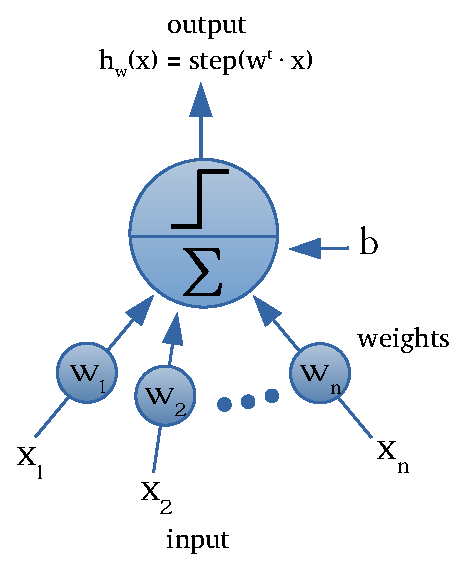
\includegraphics[scale=0.7]{{img/Perceptron2.pdf}}
	\caption{A schematic representation of a perceptron.}
	\label{fig:Perceptron}
\end{figure}

\noindent The revolutionary feature of the perceptron was the ability of learning by an adjustment of the weights. But a single perceptron is not enough this kind of logical units have lots of limitations. An example of limitation for the perceptron is shown in \figRef{fig:XORproblem} where the impossibility of implement a \textsc{xor} operation using a perceptron is shown with a graphical explanation. The perceptron is a linear classification algorithm and in the image is represented as a blue line that set a boundary for the acceptation of the hypothesis.

\begin{figure}[!htb]
	\centering
	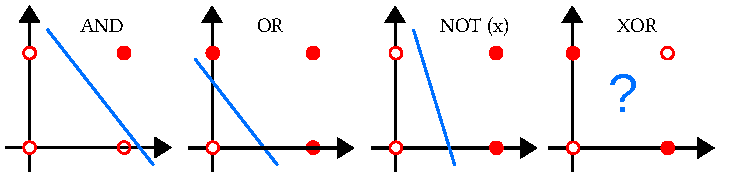
\includegraphics[width=14cm]{{img/XORproblem.pdf}}
	\caption{The figure shows one of the limitations of the perceptron. The \textsc{xor} operation is not possible with a linear cut.}
	\label{fig:XORproblem}
\end{figure}

The structure is very simple with a single unit but is not enough it have a lot of limitation so we have to introduce the concept of NN with more than one unit if we want eliminate these limitations and approximate every type of functions.

\subsection{Feed-Forward Neural Networks}

In a Neural Network different units called "neurons" are linked together. Different type of NNs exist and they are classified according to the various ways the neurons are linked together. We are interested in \textit{fully-connected Feed-Forward NNs}, that are the ones used in \textsc{mcnntunes}. 
\\
In fully-connected NNs each neurons from a layer are connected to every neurons in the next layer. While, the Feed Forward attribute refers to the fact that the NN have not internal recursions (loops) between neurons but all the neurons from a layer are connected forward to the ones of the next layer.
\\
\figRef{fig:NNesample} shows a schematic view of a fully-connected feed-forward multi-layer NN the basic idea is that the neurons can get some value in input and return a value as output. The output of neuron is then sent to all the neurons in the next layer and weighted differently for each one. 
To be more specific: each unit $j$ in the hidden layer $(i)$ takes a vector of values $x^k$, that come from all the $k$ neurons of the previous layer, and an offset $\vartheta_j$ as input, compute the weighted sum $\sum_k w_{kj}x^k$ and apply the activation function $\phi$ to the result, common choices for this function are \textit{tanh} or \textit{sigmoid}. So, the total output of the $(i)$-th layer in the network is the function:
\begin{equation}
	f^{(i)}(x) = \displaystyle\sum_{j=1}^{N^{(i)}} \varphi \left( \displaystyle\sum_k w^{(i)}_{kj}x^k + \vartheta_j^{(i)} \right)\quad,
\end{equation}
where $N^{(i)}$ is the number of hidden units in the $(i)$-th layer. 
\\ 
One of the biggest feature of the NNs is that the they are universal function approximators \cite{HORNIK1991251, LESHNO1993861} the only request for this is that a sufficient number of hidden layers is available. This is the main reason why we want use a NN based approach instead of the polynomial one
\\

\begin{figure}[!htb]
	\centering
	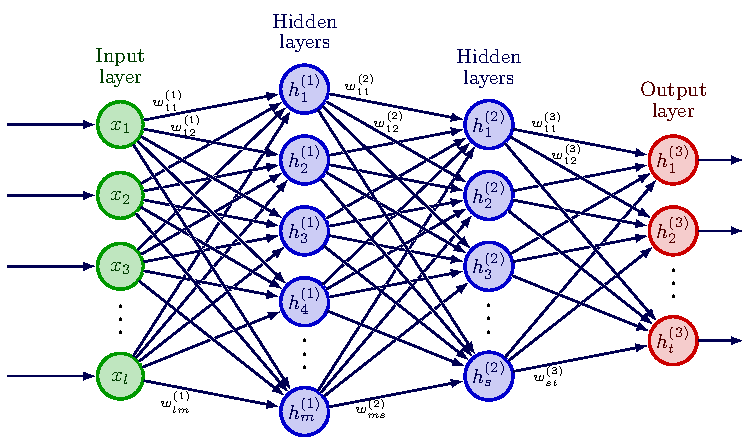
\includegraphics[width=0.95\textwidth]{{img/NN.pdf}}
	\caption{A fully-connected feed-forward neural network with more than one hidden layer, the green one is the input layer and takes the value in input and usually scale them in the range $[0,1]$ and then the data sequentially go trough the neurons in the hidden layers (blue) where all the steps described above are performed for each layer. At the end the results of the computation are collected by the output layer (red). }
	\label{fig:NNesample}
\end{figure}

\noindent As mentioned before the main feature of all the types of NNs is the ability to learn from data without being directly programmed.
But to to this and so get some predictive results from the NN a learning algorithm have to be defined.
\\
A common training algorithm for the NN is the \textit{back-propagation}. Where a set of Monte Carlo simulations is used to train the NN. The back-propagation procedure is based on the idea of change the weights, $w_{jk}$, and the offsets, $\vartheta_{j}$, in order to minimize a loss function usually defined as the mean squared error ($E$):
\begin{equation}
	E=\frac{1}{2}\displaystyle\sum_i(h_{i}(x^j,w_{jk})-d_i)^2\quad,
\end{equation}  
where the $h_{i}$ are the value in output from the NN and the $d_{i}$ the real value known from the Monte Carlo truth.
\\
In the back-propagation algorithm the weight and the coefficients are update using the \textit{steepest-descent minimization}:
\begin{equation}
	w_{jk}^{(i+1)}=w_{jk}^{(i)}-\lambda\left( \frac{\partial E}{\partial w_{jk}} \right)^{(i)}
	\quad; \ \qquad
	\vartheta_{j}^{(i+1)}=\vartheta_{j}^{(i)}-\lambda\left( \frac{\partial E}{\partial \vartheta_{j}} \right)^{(i)}
	\label{eq:learning_bp}
\end{equation}
where $\lambda$ is the learning rate and is a user-tunable free parameter. 
\\
The mini-batch are subset of our training set that contains the Monte Carlo simulations that are used to calculate the gradient. The size of the mini-batches used to train the NN is also a free parameters: smaller batches are faster to compute but the gradient direction is not the real one just an approximation; while bigger batch size give a good approximation of the direction of the steepest-descent but can be computational expensive. 
\\
The number of evaluation of the entire training set is called epochs and is tunable by the user.
\\
Note that the batch size and the number of epochs are related. A training set of 50 run with a batch size of 10 and a number of epochs of 1000 require 5000 iterations while if we use a batch size of 25 it require only 2000 iterations to run over all the training set.
\\
A schematic representation of the training process is displayed in \figRef{fig:training2} where the training set is subdivided in the mini-batches that one by one are fed to the NN. Then, the Monte Carlo truth and the output of the network are used to compute the loss function $E$, using this information the back-propagation, based on the gradient descend algorithm, updates the weights in the descent direction of the gradient calculated using the mini-batch. All the procedure is repeated with every mini-batch and for a user tunable number of epochs.

Note that the prediction capability of the Neural Network is dependent on the selection of all these user-tunable parameters that control the Neural Network architecture. All these parameters are usually referred as \textit{hyperparameters}. 

\begin{figure}[!htb]
	\centering
	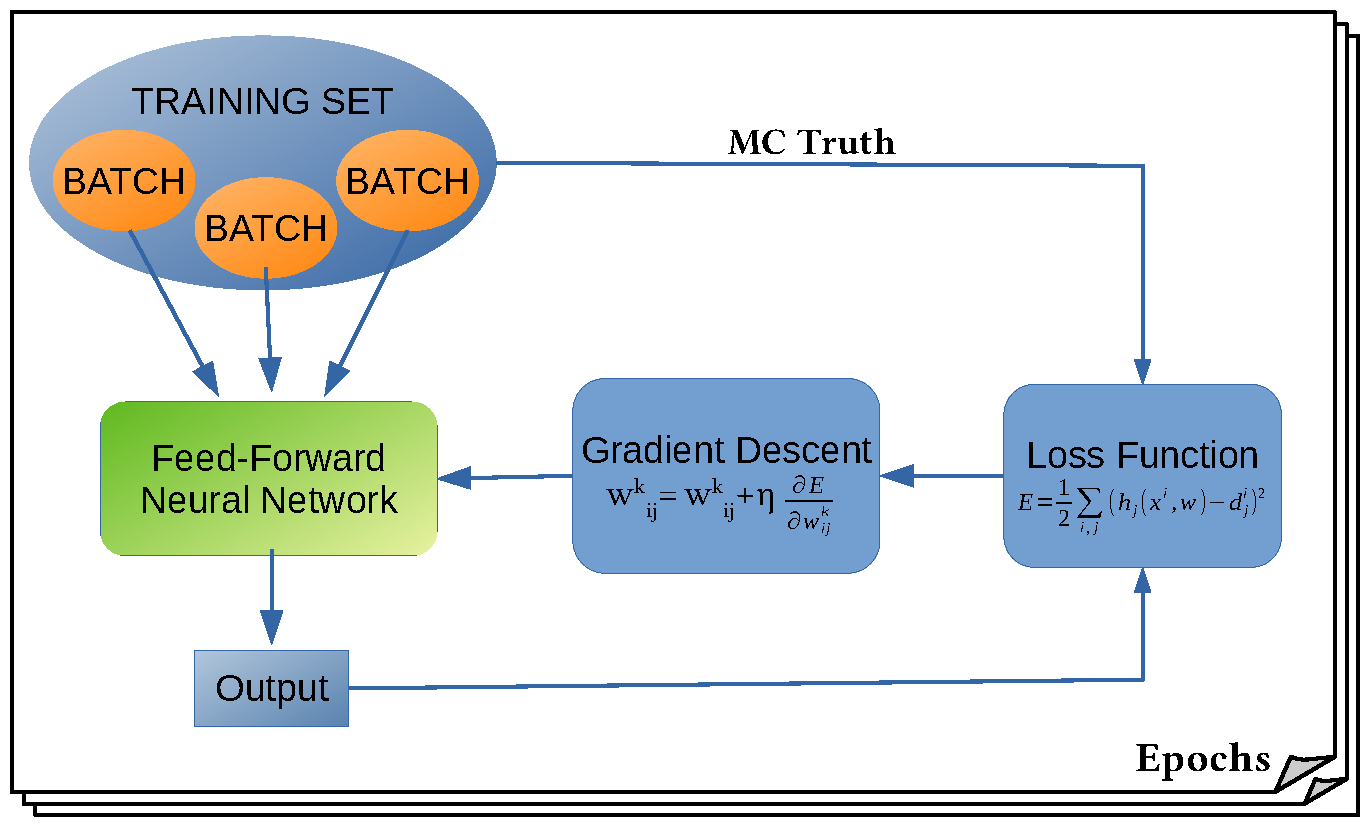
\includegraphics[width=14cm]{{img/Training2.pdf}}
	\caption{The training set used to train the NN is divided in mini-batch (the mini-batch size is a user tunable parameter) than one by one the baths are feed to the NN the output of the network together with the Monte Carlo truth are used to calculate the loss function. Then the weights and the offset are updated as described in \eqRef{eq:learning_bp} with the back-propagation algorithm. This is done with each mini-batch in the training set and for a number of epochs defined from the user. }
	\label{fig:training2}
\end{figure}


%%%%%%%\section{Previous Tune for the Underlying Event} OLD

In the next section \texttt{mcnntunes} is introduced and all its working modes are explained in detail. 

\section{MCNNTUNES}

\texttt{mcnntunes} \cite{MCNNTUNESarticle} is a Shower Monte Carlo generators tuning tool that implements a tune procedure based on the use of Feed Forward Neural Networks (FFNNs). The advantage of using FFNNs have been described above and is that they are universal function approximators at the simple cost of have a sufficient number of hidden units in the hidden layers. This feature allows us to remove the polynomial bias present in \texttt{professor} tool.
\\
\texttt{mcnntunes} offers two different main operation modes: \textit{PerBin Model} and \textit{Inverse Model}. The first one is based on approach similar to the one in \texttt{professor} but where the response of the generator is parameterized using these FFNNs, one for each bin; the later is a totally new approach where the NN (only one in this case) is trained to learn the inverse function of the generator response and then used to try to infers the parameters value starting the experimental values of the bins in the distributions used.
\\

\medskip

\subsection{Sampling Phase and Training Set Generation}

The two approach have the same starting point that is a sampling of the parameter space (e.g. for the UE analysis we use the parameters space shown in \tableRef{table:CP5variations}), than the generator is run with every sampled configuration. 
All these MC runs are going to build our dataset that is called \textit{training set}.
\\
A schematic explanation of how the sampling phase and the training set generation were performed in CMSSW environment (lxplus \textsc{cern}) is shown in \figRef{fig:worksampling}. 
In more detail the sampling start by mean of \textsc{mcnntunes} script called \textsc{mcnntemplate} with a sampling of the defined parameter space. The sampling generates  $N$ different configuration for the parameters to tune, this are then encapsulated in a runcard for \textsc{pythia} that contains all the necessary information to make \textsc{pythia} work properly (beams energies, type of event to simulate etc.). Then the \textsc{pythia} generator is run with every configuration generated and this is performed not locally but on a computers batch (e.g. the \textsc{cern} one CondorHT). The runcards we pass to Condor contain also the information on the analysis we want to performe and on how to fill the various histograms for the observables. Once the generators runs end the outputs are saved in the \textsc{yoda} format, that is a particular type of data file. The set of these \textsc{yoda} files, containing the information on the MC runs, composes our training set that then can be used for tuning procedure.

\begin{figure}[!htb]
	\centering
	\includegraphics[width=0.95\textwidth]{{img/Worksampling.pdf}}
	\caption{A schematic description of the main step from the sampling phase to the generation of the training set used for the tune procedure. These shows how the work was performed in CMSSW environment. The starting point and the final tune procedure are both controlled by \textsc{mcnntunes}. In the middle of these two phases the generation of the training set is required, this is performed running the generator many times.}
	\label{fig:worksampling}
\end{figure}

\medskip

\textsc{mcnntunes} offer also the possibility of change the value of the hyperparameters. The value that can be modified for the Neural Network. It is possible to chose the NN architecture: the number of hidden layer, the number of neurons for each layer and the activation function used. It is also possible to set the number of epochs, the batch size and the learning rate in order to have the best train for the architecture selected and other choice are possible. This is really important in order to get the best possible results for the tune.

\subsection{Per Bin Model}
\label{sec:PerBinModel}

PerBin Model is a parametrisation-based method. The main idea, as shown in \figRef{fig:PerBinModel_schematic} is to build a model (i.e. a neural network) for each bin in order to parameterize the generator output. Each NN takes the parameters values as input and returns the bin value as output.
\\
All these NNs are then trained feeding the MC runs from the training set and  using a gradient-based algorithm, as usual for feed forward neural networks, with mean squared errors as loss function.
\\
Once, the NN is trained, the last step is the tune in which one actually get the best parameters estimation.  This step define a surrogate loss function for the tuning problem. In fact, the parameterization step return a model $h^{(i)}(\mathbf{p})$ for each bin, $i$, where $\mathbf{p}$ is the vector of the parameters. 
\\
Then, this surrogate loss function defined as:
\begin{equation}
	\chi^2=\displaystyle\sum_{i=1}^N\frac{\left( h^{(i)}(\mathbf{p})-h_{exp}^{(i)}\right)^2}{\sigma_{(i)}^2}
\end{equation}
need to be minimized in order to evaluate the best estimation for the parameters. In \texttt{mcnntunes} this minimization is performed using the CMA-ES algorithm \cite{CMAES}.
\\
So the best estimation for the parameters is the configuration of parameters that minimize this $\chi^2$.  

\begin{figure}[!htb]
	\centering
	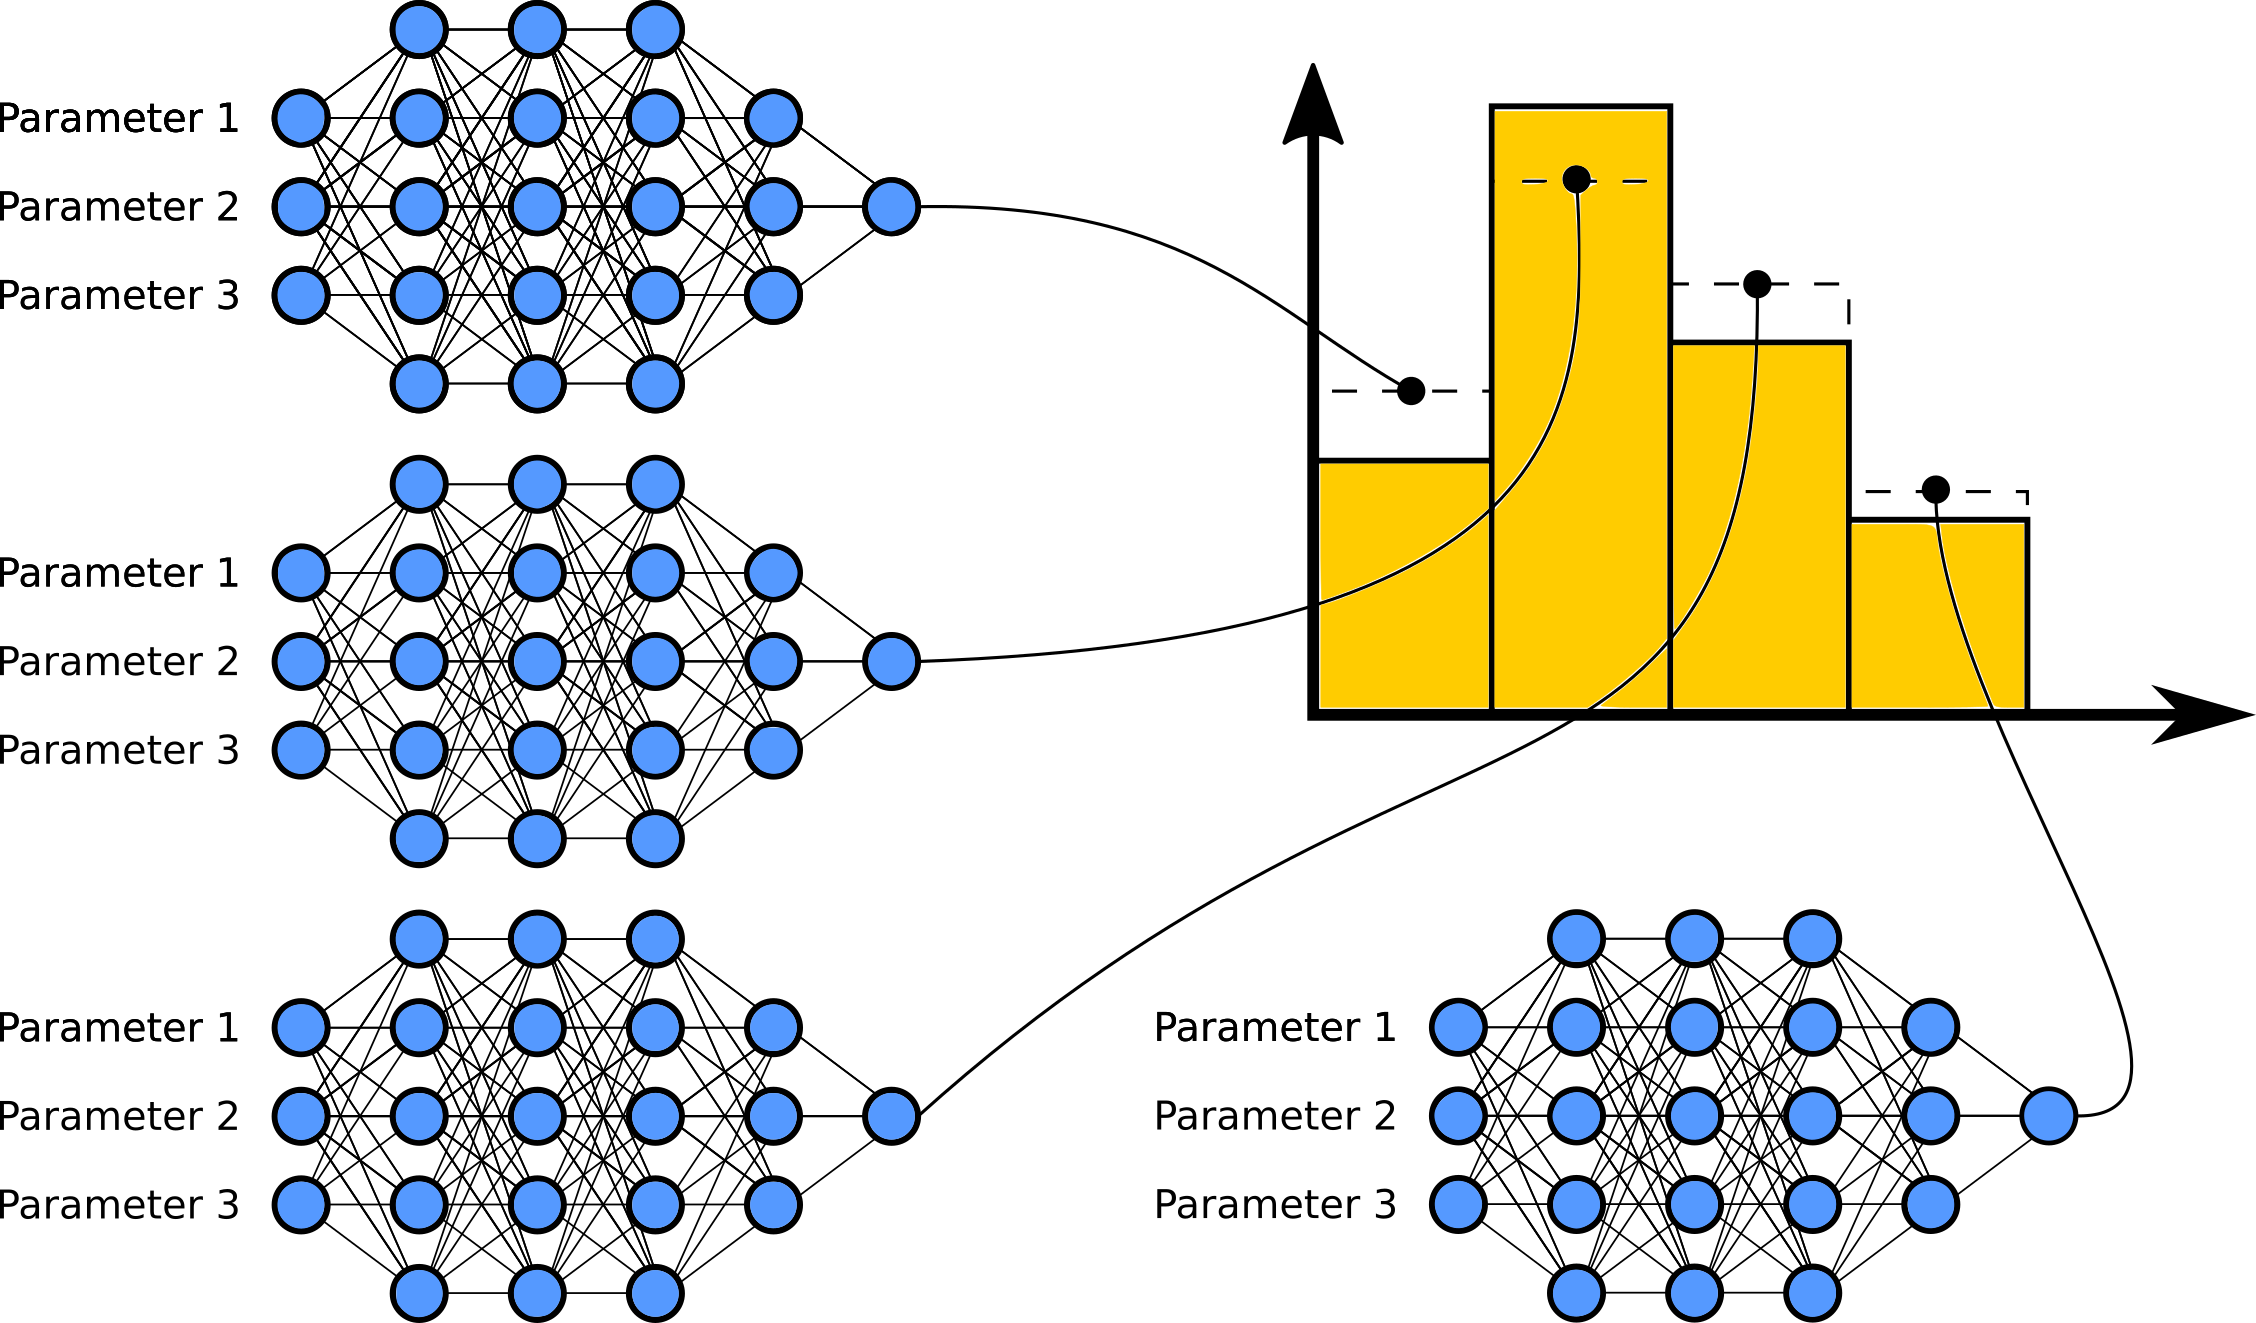
\includegraphics[width=0.8\textwidth]{{img/PerBinModel.png}}
	\caption{Figure from \cite{MCNNTUNESarticle}}
	\label{fig:PerBinModel_schematic}
\end{figure}

\subsubsection{Errors evaluation}

\textsc{mcnntunes} PerBin model as introduced in \cite{MCNNTUNESarticle} did not have a proper error evaluation. In fact it was using as error the final width of the distribution of sampled point in the CMA-ES algorithm. But, this was not working. Thanks to S. Carazza and with the help of M. Lazzarin we had the opportunity of handle the code and add a proper errors estimation.

Now, the errors evaluation for the PerBin Model is given by the definition of a confidence interval using the $\chi^2$ function.
In fact, as shown in section 9.6 and 9.7 of \cite{cowan}, for an estimators vector $\hat{h}(\mathbf{p})=(\hat{h}^{(1)}(\mathbf{p}),\hat{h}^{(2)}(\mathbf{p}),\dots,\hat{h}^{(n)}(\mathbf{p}))$ for the parameters $\mathbf{p}$ the probability distribution function and the likelihood (the $\chi^2$ in our case) in limit of a large sample\footnote{In other case this still a good approximation.} are Gaussian distributed. The probability distribution function for the estimators is than:
\begin{equation}
f(\hat{h}(\mathbf{p})|h(\mathbf{p})) = \frac{1}{(2\pi)^{n/2}|V|^{1/2}}\exp\left[ -\frac{1}{2}\left(\hat{h}(\mathbf{p}) - h(\mathbf{p})\right)^T V^{-1} \left(\hat{h}(\mathbf{p}) - h(\mathbf{p})\right) \right] \ ,
\end{equation}
where $T$ is the transpose vector and $V^{-1}$ is the inverse covariance matrix. 
Can be shown that also the likelihood is Gaussian as the probability distribution function. 
%So a changing in the parameter give a calculable variation in the $\chi^2$
So, we can define our confidence interval using the $\chi^2$ statistic as: 
\begin{equation}
	\frac{\chi^2(\text{c.i.})}{N_{dof}}= \frac{\chi^2_{min}}{N_{dof}}+\frac{Q_\gamma}{N_{dof}}
	\label{eq:chi2_variation}
\end{equation} 
The variation is dependent on the number of parameters and on the chosen confidence level ($1\sigma=0.683$ in our case) and a list of the values is reported in \tableRef{table:percentile}.

\begin{table}
	\centering
	\begin{tabular}{c | c c c c c}
		\multirow{ 2}{*}{percentile} & \multicolumn{5}{c}{$Q_\gamma$}\\\cline{2-6}
		& $n=1$ & $n=2$ & $n=3$ & $n=4$ & $n=5$ \\\hline\hline
		$0.683$& $ 1.00 $ & $ 2.30 $ & $ 3.53 $ & $ 4.72 $ & $ 5.89 $ \\
		$0.90$ &  $ 2.71 $ & $ 4.61 $ & $ 6.25 $ & $ 7.82 $ & $ 9.24 $ \\
		$0.95$ & $ 3.84 $ & $ 5.99 $ & $ 7.82 $ & $ 9.49 $ & $ 11.1 $ \\
		$0.99$ & $ 6.63 $ & $ 9.21 $ & $ 11.3 $ & $ 13.3 $ & $ 15.1 $ \\
	\end{tabular}
	\caption{The table report the values of the quantile $Q_\gamma$ for different confidence level $0.683$ is the row corresponding to the $1\sigma$ definition and is the one of our interest.}
	\label{table:percentile}
\end{table}

\noindent Then, the error is defined as the value of the parameters that give a deviation from the minimum value of the $\chi^2/N_{dof}$ equal to the $Q_\gamma/N_{dof}$ value for a confidence level of $0.683$, as defined in \eqRef{eq:chi2_variation}.
\\
An example for the evaluation in \texttt{mcnntunes} is shown in \figRef{fig:exampleChi2Variation} where the green line is the deviation from the minimum value of the $\chi^2$ defined in \eqRef{eq:chi2_variation} and the errors are given by the points where the $\chi^2/DoF$ reach these value. Therefore, the intersections between green and blue line that is the $\chi^2/N_{dof}$ for the different values of the parameter.

\begin{figure}[!htb]
	\centering
	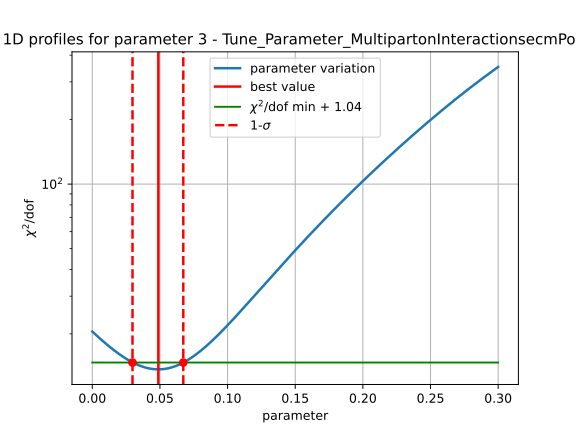
\includegraphics[width=0.6\textwidth]{{img/exampleChi2Variation.png}}
	\caption{This figure shows the error evaluation in \texttt{mcnntunes} for the \texttt{MultipartonInteractions:ecmPow} \texttt{Pythia8} parameter. The blue line is the value of the $\chi2/N_{dof}$ evaluated for different parameter values. The best estimation is indicated by the vertical red line, while the green line is the quantity in \eqRef{eq:chi2_variation}. The error is evaluated from the intersection of blue and green lines.
	}
	\label{fig:exampleChi2Variation}
\end{figure}

\subsection{Negative aspects}

One of the negative aspect is that this model is more computational expensive than the below discussed Inverse model. This is due to the large number of NNs built and trained from this model. 
The high cost in term of time required to get the model work do not give the possibility for a scan in the hyperparameters space in order to obtain the best configuration for the NN architecture. 
\\
This can impose some limitation on the model performance that cannot get its maximum  performance.

\subsection{Inverse Model}

The Inverse Model is the most innovative tuning procedure introduced by \texttt{mcnntunes}. This model contrarily to the PerBin Model takes the histograms bins as input and returns parameters values as output. For the Inverse Model the NN used is only one as shown schematically in \figRef{fig:InverseModel_schematic}. What the Inverse Model try to do is to learn the inverted model of the generator. So starting from the observed values the model try to reproduce the parameters values necessary to get the histograms we use as input.

The model is build and then trained with the training set introduced before. Once the model is trained feeding the experimental data to the NN this can try to infer the values of the parameters required to get the output. 

\begin{figure}[!htb]
	\centering
	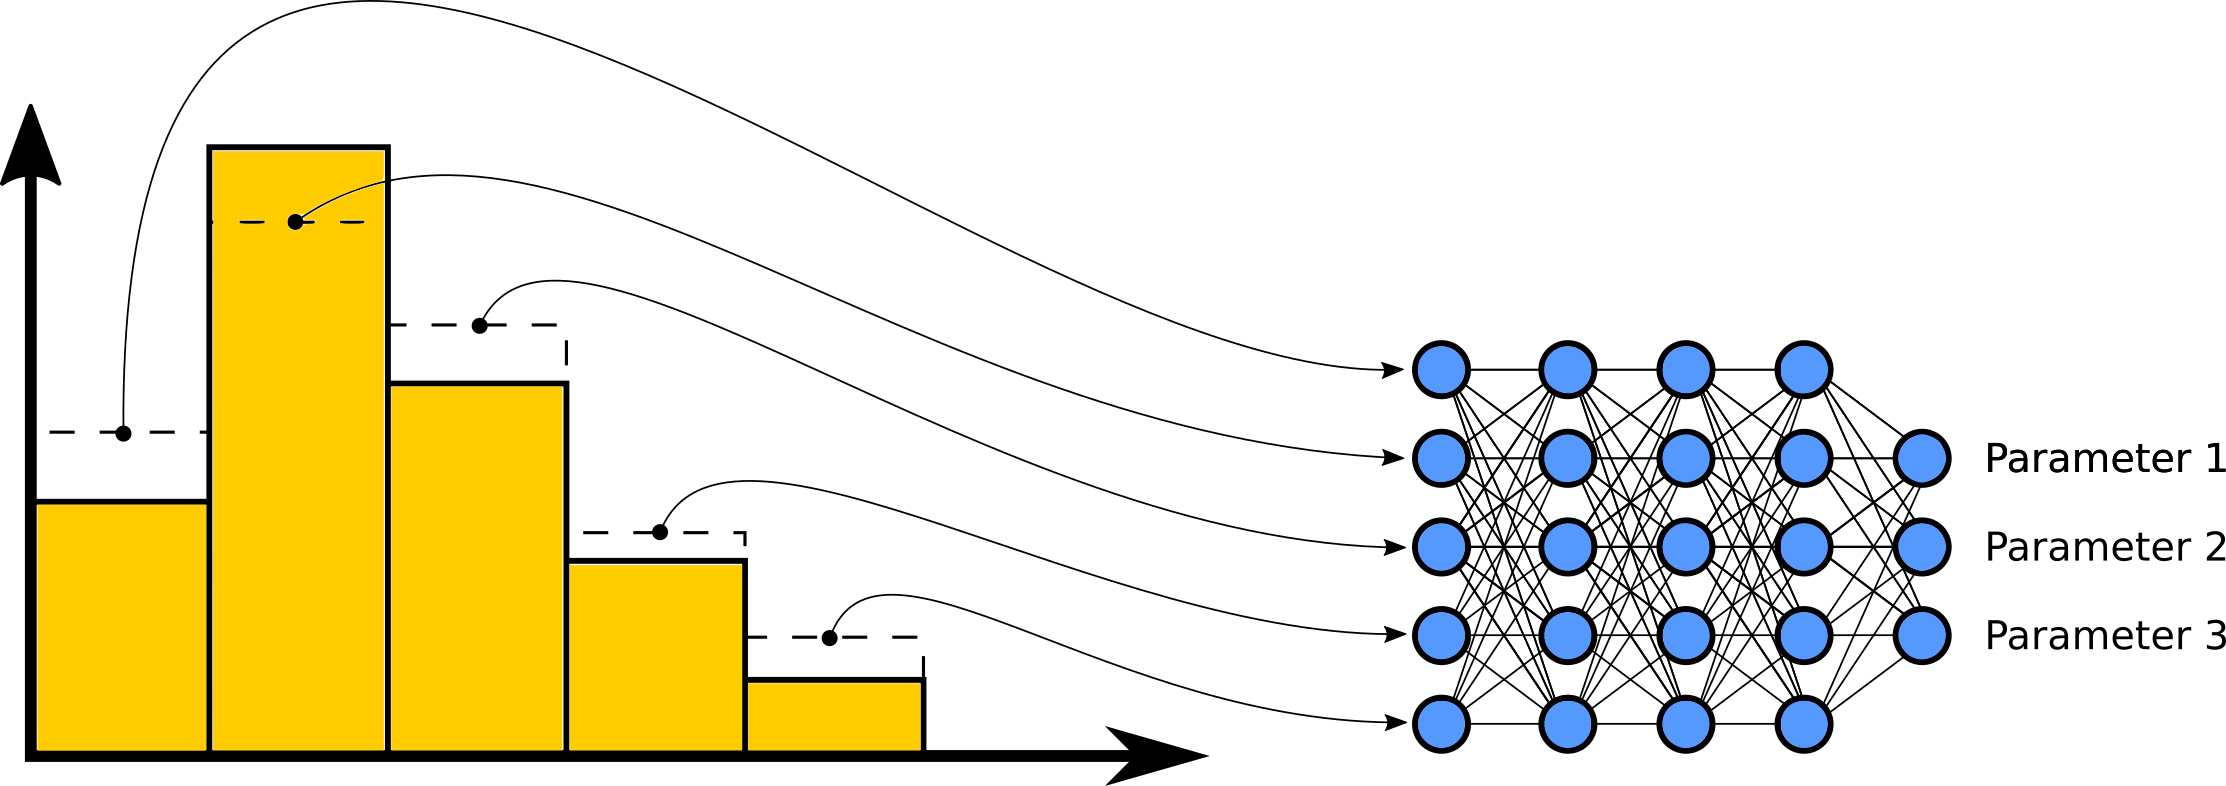
\includegraphics[width=0.8\textwidth]{{img/InverseModel.png}}
	\caption{Figure from \cite{MCNNTUNESarticle}}
	\label{fig:InverseModel_schematic}
\end{figure}

\subsubsection{Errors evaluation}

The errors are evaluated in a different way respect to PerBin Model in fact in the Inverse Model there is not a minimization step, and the error is evaluated by a re-sampling of the experimental data using a \textit{multivariate Gaussian Distribution}, as in \eqRef{eq:gaussianDristribution} with a diagonal covariance matrix that have experimental uncertainties on the main diagonal.
\begin{equation}
	f(x_i; h^{(i)}_{\text{exp}}, \sigma^{(i)}_{\text{exp}})\,=\,\mathcal{N}\cdot\exp\left[ 
	-\frac{1}{2}
	\displaystyle\sum_{j=1}^{N_{bins}}
	\frac{\left( 
	x_i - h^{(i)}_{\text{exp}} 
	\right)^2}{{\sigma^{(i)}_{\text{exp}}}^2} 
	\right]
	\label{eq:gaussianDristribution}
\end{equation}
So, a set of histograms is generated, then this is fed to the NN and a distribution of predictions is generated. An example is shown in \figRef{fig:InverseModel_predictionsSpread}, from this distribution one can compute the error by evaluating the standard deviation.

\begin{figure}[!htb]
	\centering
	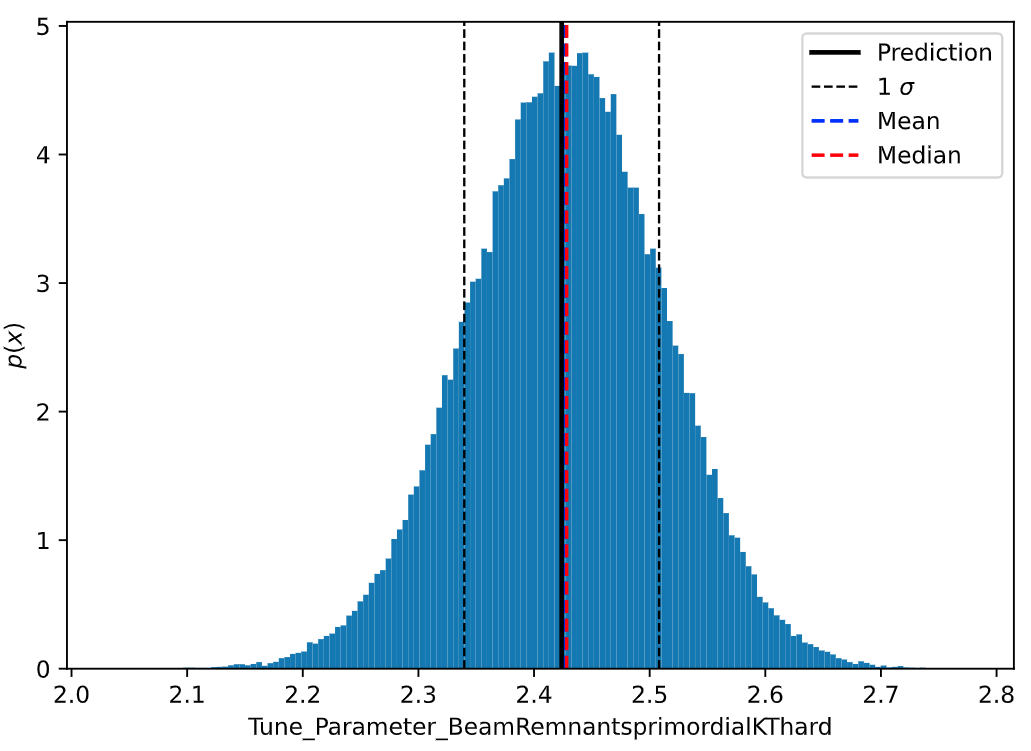
\includegraphics[width=0.6\textwidth]{{img/InverseModel_predictionsSpread.png}}
	\caption{Predictions spread for the inverse model after that a Gaussian resample is performed}
	\label{fig:InverseModel_predictionsSpread}
\end{figure}

Note that this is a new method for the tune. As we are going to see this method requires more attentions than the PerBin Model to get it working correctly in the case of an high number of parameters to tune.

Respect to the PerBin Model this method is faster. The NN trained is only one and is not needed a minimization so a scan in the hyperparameters can be performed in order to search for the best architecture. 

 
\subsubsection{Hyperparameters}

A really important step in the Inverse model is the \textit{hyperparameter optimization} it is required to get the method working. 

The procedure consist in build a \textit{validation set } containing some Monte Carlo simulations as the training set (e.g. $10\%$ of the simulations in the training set) and retrain the model with different choices for the NN architecture. Than a closure test is performed in order to estimate the performance of the NN and then the best model is retrained and the experimental data are fed to it in order to get the best estimation for the parameters to tune. This procedure is schematically summarized in \figRef{fig:HyperParams}.
\\
The hyperparameters scan is performed using the python package \texttt{hyperopt}.


\begin{figure}[!htb]
	\centering
	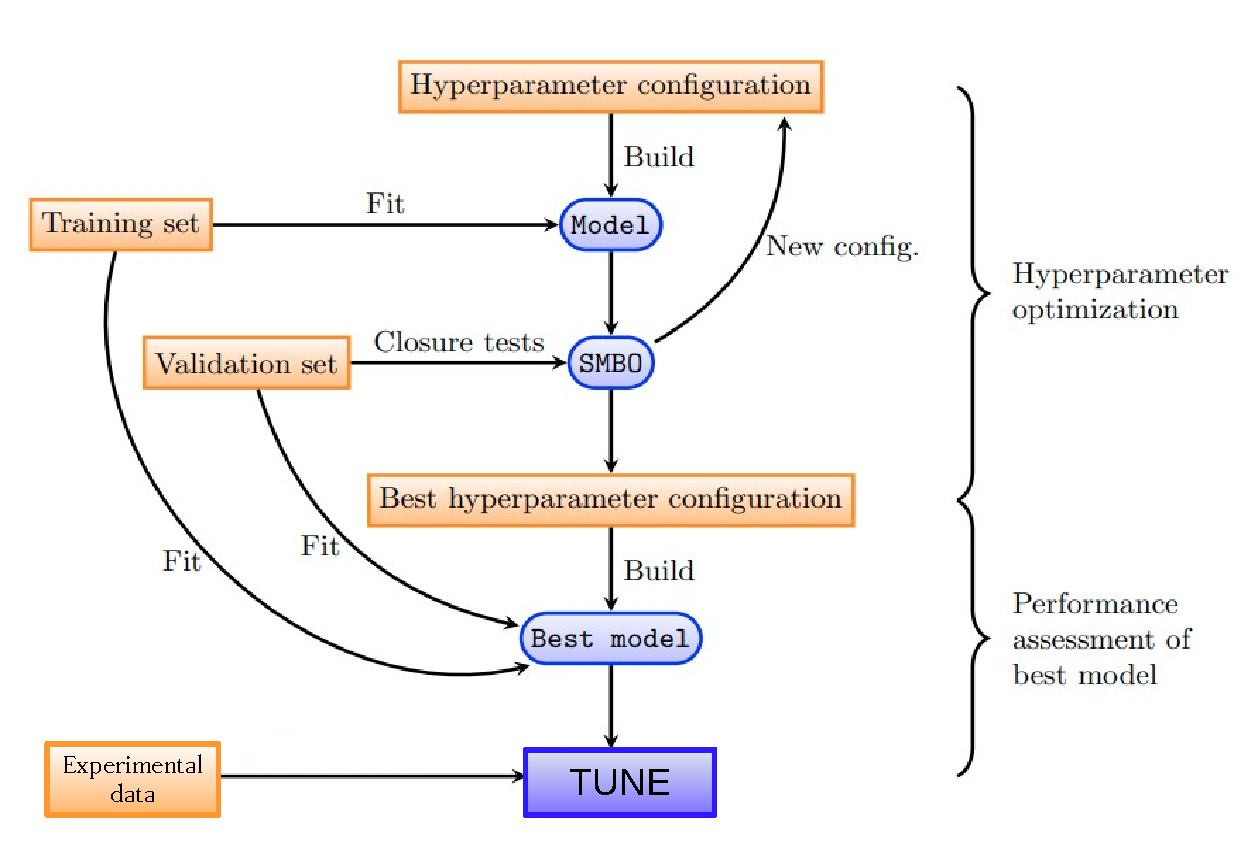
\includegraphics[width=0.9\textwidth]{{img/workflow.pdf}}
	\caption{The hyperparameter optimization procedure is schematically shown here. The model is trained using a training set than performing a closure test a scan on the hyperparameter is done. Once the best configuration is found the best model is retrained using both the runs in the training set and the runs in the validation set. Then the experimental data are fed the network and the best parameters are estimated. Figure from \cite{MCNNTUNESarticle}}.
	\label{fig:HyperParams}
\end{figure} 

\subsubsection{Problems}

As we are going to see the main problem for the Inverse model is the stability in the results. The operation that this model is trying to do is very hard, learn the inverse response of the generator is not an easy task. This difficulties in some case leads to a bad prediction. 
\\
As we are going to see in the chapter on our tune the inverse model requires some more attention than the PerBin model to get it work properly and in some case when the number of parameters became large and maybe the correlation between the parameters are important this model fails. 
\\
But if more care are given to this model this can become a very powerful method for future tunes.


\subsection{Weightrules in MCNNTUNES}

\textsc{mcnntunes} as \textsc{professor} implement the possibility of change the weight of the singles bins in the distributions. This is a really useful feature. As we will discuss later we use these weightrules to get a results more similar to CP5 in our tune. Increasing the weight of a bin this bin became more important in the overall $\chi^2$ evaluation and it is better described by the simulations. An example is shown in \figRef{fig:CMS_weightrules} where the application of the weightrules takes us to a better description of the experimental data.

\begin{figure}[!htb]
\centering
\noindent
	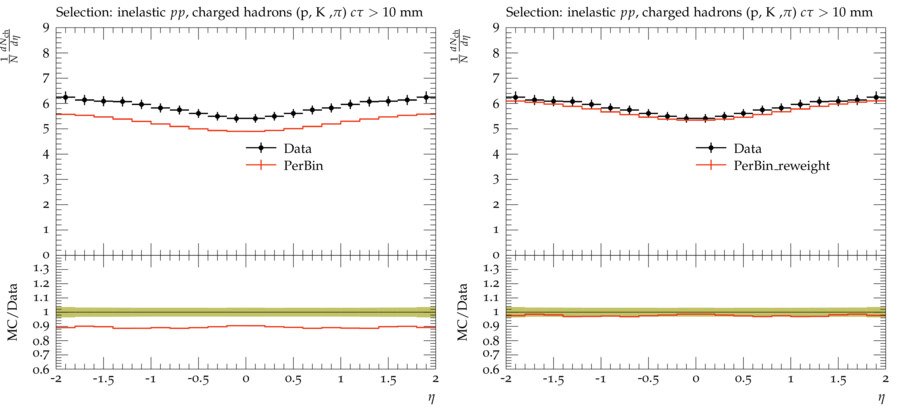
\includegraphics[width=0.85\textwidth]{{img/CMS2015_weightrules.jpg}}
	\caption{An example of weightrules application. Here the black point are the experimental data from the CMS analysis at $\sqrt{s}=13\ \mathrm{TeV}$ \cite{CMS:2015zrm} while the colored lines are the simulations, the vertical lines on MC points indicate the statistical uncertainties. It is easy to see that the distribution in the right panel is not well described from the tune, but thanks to the weightrules we can give to this distribution a greater importance in the tune and describes it better as shown in the left panel. This is better explained in the next chapter.}
	\label{fig:CMS_weightrules}
\end{figure}   


